% !TEX encoding = UTF-8 Unicode

\documentclass{article}
\usepackage[french]{babel}
\author{Louis DESVERNOIS, Alexis SCHOENN, Philippe DUBOIS}
\title{%
    SAÉ24: Web \\
    \large Groupe 13}
% \date{9 Juin 2022}
\usepackage[left=2.5cm,right=2.5cm,top=2.5cm,bottom=2.5cm]{geometry}
\usepackage{subcaption}
\usepackage{listings}
\usepackage{minted}
\usepackage{graphicx}
\usepackage[T1]{fontenc}
\usepackage[colorlinks=true,linkcolor=black,anchorcolor=black,citecolor=black,filecolor=black,menucolor=black,runcolor=black,urlcolor=black]{hyperref}

%\setcounter{tocdepth}{1} % pour la profondeur de la ToC

\usepackage{fancyhdr}
\pagestyle{fancy}
\fancyhf{}
\renewcommand{\headrulewidth}{0pt}
\rfoot{\thepage}
\lfoot{SAÉ24: Groupe 13}

\renewcommand{\listoflistingscaption}{Table des codes}
\renewcommand{\listingscaption}{Code}

\begin{document}

\maketitle
\tableofcontents
\listoffigures
\listoflistings

\newpage
\section{Introduction}
Nous avons créé un site web dynamique avec le framework Django pour afficher les données récupérées par le script de collecte MQTT.
Notre site doit être capable d'afficher les données avec plusieurs filtres et nous devons être capables de modifier le nom et l'emplacement de chaque capteurs.

\section{Base de données}
\subsection{Mise en place du serveur MySQL}
Nous avons utilisé MySQL Workbench pour créer le serveur ainsi que pour le configurer.
Workbench n'est qu'une interface graphique à MySQL, mais n'est pas nécessaire une fois le serveur configuré.
Pour commencer il faut installer le serveur MySQL sur notre machine Windows en le téléchargeant sur le site officiel de MySQL, le programme est activé automatiquement.
Une fois le serveur installé et activé nous devons nous connecter avec Workbench.
\begin{figure}[H]
    \begin{center}
        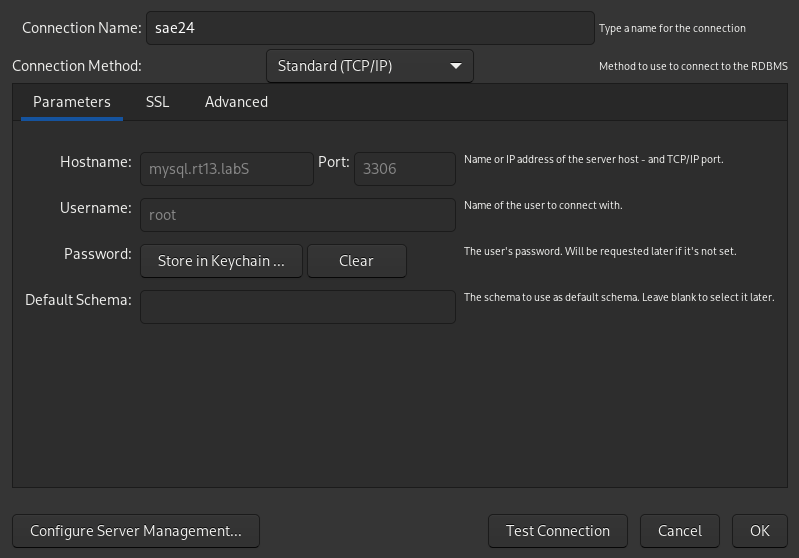
\includegraphics[width=0.7\linewidth]{fig/workbench-conn.png}
    \end{center}
    \caption{Connexion à la BDD avec Workbench}
    \label{workbench:conn}
\end{figure}
Dans la Figure \ref{workbench:conn}, le serveur MySQL est déjà configuré pour accepter les connexions extérieures, pour activer cela, il faut naviguer dans le menu \emph{Server} puis \emph{Users and Privileges} et configurer le paramètre \emph{Limit to Host Matching} pour le bon utilisateur. En Figure \ref{workbench:ip-matching} nous avons configuré l'accès au VLAN server uniquement avec le \emph{wildcard} \verb|%|.
\begin{figure}[H]
    \begin{center}
        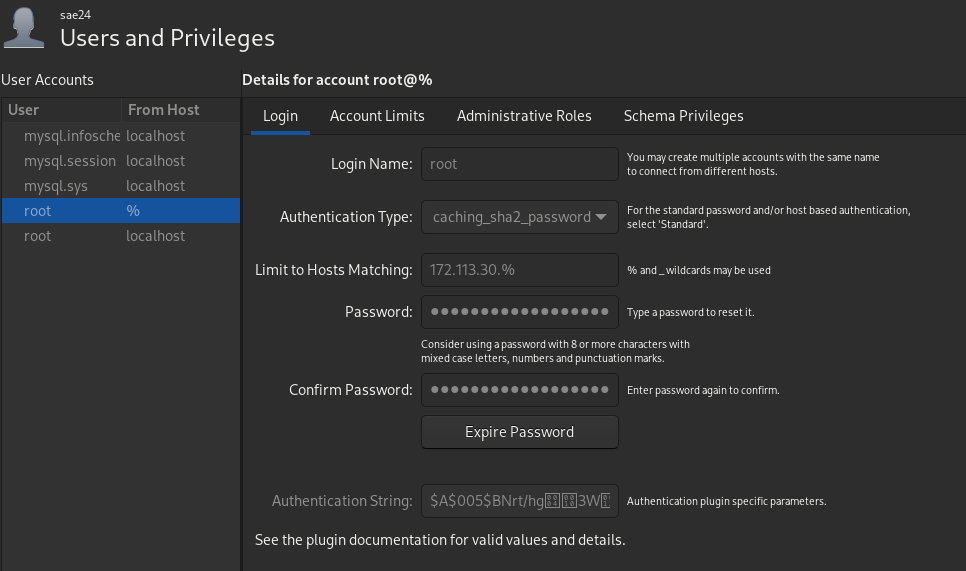
\includegraphics[width=0.7\linewidth]{fig/workbench-allow-ip.png}
    \end{center}
    \caption{Paramétrage de l'accès à distance}
    \label{workbench:ip-matching}
\end{figure}

\subsection{Création de la base de données et des tables}
La base de données ainsi que les tables sont créés dans notre script de collecte MQTT avec des requêtes SQL.
\begin{listing}[H]
    \begin{minted}[breaklines]{sql}
CREATE DATABASE temp;
USE temp;

CREATE TABLE IF NOT EXISTS temp.sensors (
    id INT NOT NULL AUTO_INCREMENT,
    macaddr VARCHAR(12) NOT NULL,
    piece VARCHAR(50) NOT NULL,
    emplacement VARCHAR(50),
    nom VARCHAR(50),
    UNIQUE (macaddr),
    PRIMARY KEY (id));

CREATE TABLE IF NOT EXISTS temp.sensors_data (
    id INT NOT NULL AUTO_INCREMENT,
    sensor_id INT NOT NULL,
    CONSTRAINT sensorFK
        FOREIGN KEY (sensor_id)
        REFERENCES temp.sensors(id),
    datetime DATETIME NOT NULL,
    temp FLOAT NOT NULL,
    PRIMARY KEY (id));
    \end{minted}
    \caption{Création de la base de données et des tables}
    \label{bdd:creation}
\end{listing}

\section{Création projet Django}
\subsection{Initialisation}
Pour commencer, nous avons besoin d'initialiser notre projet Django.
Pour cela nous allons d'abord créer un environnement virtuel Python avec la commande \verb|python3 -m venv .venv| nous pouvons ensuite l'activer avec \verb|source .venv/bin/activate|.
Une fois dans l'environnement virtuel, nous pouvons utiliser \verb|pip install| pour installer les paquets dont nous avons besoin, c'est-à-dire django, django-admin et mysqlclient\footnote{Nous avons également besoin d'installer le paquet mariadb-clients avec apt pour que l'installation fonctionne}.
Avec tous les paquets installer, nous pouvons, exécuter les commandes \verb|django-admin startprojet sae24| pour initialiser le projet et \verb|django-admin startapp temp| pour créer l'application.

\subsection{Connexion de Django à la base de données}
Pour connecter Django à notre de base de données, nous devons modifier le fichier \verb|settings.py| du projet.
\begin{listing}[H]
    \begin{minted}[breaklines]{python}
DATABASES = {
    'default': {
        'ENGINE': 'django.db.backends.mysql',
        'NAME': 'temp',
        'USER': 'root',
        'PASSWORD': 'admin',
        'HOST': 'mysql.rt13.lab',
        'PORT': '3306',
    }
}
    \end{minted}
    \caption{settings.py: connexion à la BDD}
    \label{django:bddconn}
\end{listing}
Maintenant que nous sommes connectés à la base de données nous pouvons créer automatiquement le fichier \verb|models.py| en utilisant la commande \verb|./manage.py inspectdb > temp/models.py|.

\subsection{Création du form}
Nous pouvons maintenant créer le form pour les capteurs, qui nous permet de modifier le nom et l'emplacement du capteurs.
\begin{listing}[H]
    \begin{minted}[breaklines]{python}
class SensorsForm(ModelForm):
    class Meta:
        model = models.Sensors
        fields = ('emplacement', 'nom')
        labels = {
            'nom': 'Nom',
            'emplacement': 'Emplacement'
        }
    \end{minted}
    \caption{Formulaire pour les capteur}
    \label{django:form}
\end{listing}
En code \ref{django:form} nous n'ajoutons pas les fields qui ne doivent pas changer dans la base de données.

\newpage
\subsection{Création des views}
Maintenant que notre formulaire est créé, nous pouvons nous atteler à la création des views de notre projet.
\subsubsection{Affichage}
Les views d'affichage sont les plus simples à créer, en effet, il suffit de récupérer tous les objets d'un models et de les envoyer dans les templates HTML.
\begin{listing}[H]
    \begin{minted}[breaklines]{python}
global refresh
global refresh_time
refresh = True
refresh_time = 20

def liste_sensors(request):
    sensors = Sensors.objects.all()
    return render(request, 'sensors/liste.html', {'sensors': sensors})

def liste_data(request):
    data = SensorsData.objects.all()
    return render(request, 'data/liste.html', {'data': data, 'refresh': refresh, 'refresh_time': refresh_time})
    \end{minted}
    \caption{Views d'affichage}
    \label{django:views:affichage}
\end{listing}
Les variables \verb|refresh| et \verb|refresh_time| permettent d'activer ou de désactiver le rafraîchissement automatiquement. 
Les deux templates appelées ici sont quasiment identique, les seules différences sont le nombre de colonnes dans le tableau.

\subsubsection{Modification}
La modification des capteur se fait avec deux views, un de modification qui affiche le formulaire (code \ref{django:views:modif1}) et un autre qui enregistre les modifications dans la base de données (code \ref{django:views:modif2}).
\begin{listing}[H]
    \begin{minted}[breaklines]{python}
def modif_sensors(request, id):
    obj = Sensors.objects.get(id=id)
    objform = SensorsForm(model_to_dict(obj))
    if request.method == "POST":
        form = SensorsForm(request.POST)
        if form.is_valid():
            form.save()
            return HttpResponseRedirect("/sensor/liste")
    else:
        return render(request, "sensors/modif.html", {"form": objform, "id": id})
    \end{minted}
    \caption{Views de Modification 1}
    \label{django:views:modif1}
\end{listing}

\begin{listing}[H]
    \begin{minted}[breaklines]{python}
def save_modif_sensors(request, id):
    objform = SensorsForm(request.POST)
    bak = Sensors.objects.get(id=id)
    sensors = Sensors.objects.all()
    if objform.is_valid():
        objform = objform.save(commit=False)
        objform.id = id
        objform.macaddr = bak.macaddr
        objform.piece = bak.piece
        for i in sensors:
            if i.nom == objform.nom:
                return HttpResponseRedirect(f"/sensors/modif/{id}")
        objform.save()
        return HttpResponseRedirect("/sensors/liste")
    else:
        return render(request, "sensors/modif.html", {"form": objform, "id": id})
    \end{minted}
    \caption{Views de Modification 2}
    \label{django:views:modif2}
\end{listing}
En code \ref{django:views:modif2}, nous créons une copie du capteur que nous souhaitons modifier sans cela, notre bouton modifier supprimerais l'adresse MAC et la pièce du capteur modifié, car notre form ne contient pas ces informations.

\subsubsection{Views de Filtre}
Pour créer des filtres facilement, nous pouvons utiliser la fonction \verb|filter()| des objets de model Django. Le filtre le plus simple est celui en code \ref{django:views:filtre1}, qui permet de filtrer les données par capteur.
\begin{listing}[H]
    \begin{minted}[breaklines]{python}
def filtre_par_sensor(request, id):
    data = SensorsData.objects.filter(sensor = id)
    return render(request, 'data/liste.html', {'data': data})
    \end{minted}
    \caption{Filtre par capteur}
    \label{django:views:filtre1}
\end{listing}

Nous pouvons cependant créer d'autres filtres plus complexes, par exemple, nous pouvons filtrer entre deux dates utilisant \verb|__range| et des objets \verb|datetime|. La création d'une template contenant un \verb|<form>| HTML est nécessaire.
\begin{listing}[H]
    \begin{minted}[breaklines]{html}
<form method="post" action="/data/liste_filtre">
    
    <input type="datetime-local" class="form-control" id="startDate" name="startDate" placeholder="Date de début">
    <input type="datetime-local" class="form-control" id="endDate" name="endDate" placeholder="Date de fin">
    <input type="submit" class="btn btn-success" value="Valider">
</form>
    \end{minted}
    \caption{Template de filtre entre deux dates et heures}
    \label{template:filtre}
\end{listing}

\begin{listing}[H]
    \begin{minted}[breaklines]{python}
def filtre_par_date(request):
    start = datetime.fromisoformat(request.POST["startDate"])
    end = datetime.fromisoformat(request.POST["endDate"])
    data = SensorsData.objects.filter(datetime__range=(start, end))
    return render(request, 'data/liste.html', {'data': data, 'refresh': False})
    \end{minted}
    \caption{Filtre entre deux dates et heures}
    \label{django:views:filtre2}
\end{listing}
Nous pouvons également utiliser ces deux filtres en même temps en mettant en argument les deux conditions.

\begin{listing}[H]
    \begin{minted}[breaklines]{python}
def filtre_par_date_et_capteur(request, id):
    start = datetime.fromisoformat(request.POST["startDate"])
    end = datetime.fromisoformat(request.POST["endDate"])
    data = SensorsData.objects.filter(datetime__range=(start, end), sensor = id) 
    return render(request, 'data/liste.html', {'data': data, 'refresh': False})
    \end{minted}
    \caption{Filtre par date et par capteur}
    \label{django:views:filtre3}
\end{listing}

\end{document}